%                      Code_Saturne version 1.3
%                      ------------------------
%
%     This file is part of the Code_Saturne Kernel, element of the
%     Code_Saturne CFD tool.
% 
%     Copyright (C) 1998-2007 EDF S.A., France
%
%     contact: saturne-support@edf.fr
% 
%     The Code_Saturne Kernel is free software; you can redistribute it
%     and/or modify it under the terms of the GNU General Public License
%     as published by the Free Software Foundation; either version 2 of
%     the License, or (at your option) any later version.
% 
%     The Code_Saturne Kernel is distributed in the hope that it will be
%     useful, but WITHOUT ANY WARRANTY; without even the implied warranty
%     of MERCHANTABILITY or FITNESS FOR A PARTICULAR PURPOSE.  See the
%     GNU General Public License for more details.
% 
%     You should have received a copy of the GNU General Public License
%     along with the Code_Saturne Kernel; if not, write to the
%     Free Software Foundation, Inc.,
%     51 Franklin St, Fifth Floor,
%     Boston, MA  02110-1301  USA
%
%-----------------------------------------------------------------------
%
%%%%%%%%%%%%%%%%%%%%%%%%%%%%%%%%%%
%%%%%%%%%%%%%%%%%%%%%%%%%%%%%%%%%%
\section{Discr\'etisation}
%%%%%%%%%%%%%%%%%%%%%%%%%%%%%%%%%%
%%%%%%%%%%%%%%%%%%%%%%%%%%%%%%%%%%
\subsection{\bf Partie convective}
En s'inspirant des notations adopt\'ees dans le sous-programme \fort{navsto}, le  bilan explicite correspondant \`a l'int\'egration sur une cellule $\Omega_i$
de la partie convective $-{\dive(\,(\rho\,\vect{u})^n  a)}$ de $\mathcal{B_{\mathcal{\beta}}}$ 
 peut s'\'ecrire sous forme
d'une somme de flux num\'eriques $F_{\,ij}$ calcul\'es aux faces des
cellules purement internes et de flux num\'eriques $F_{\,b_{ik}}$
calcul\'es aux faces de bord du domaine $\Omega$.
Soient $Vois(i)$ l'ensemble des centres des cellules voisines de ${\Omega_i}$ et
$\gamma_b(i)$ l'ensemble des centres des faces de bord de ${\Omega_i}$, s'ils existent. On a donc~:

\begin{equation}\notag
\int_{\Omega_i}{\dive( (\rho \vect{u})^n  a )\, d\Omega} = 
\sum_{j\in Vois(i)}{F_{\,ij}((\rho \vect{u})^n, a)} 
+\sum_{k\in {\gamma_b(i)}} {F_{\,{b}_{ik}}((\rho \vect{u})^n,a)}
\end{equation}

en posant : 
\begin{equation}
F_{\,ij}((\rho \vect{u})^n,a) = \left[{(\rho \vect{u})_{\,ij}^n} \text{.}\, \vect{S}_{\,ij}\right]\ a_{\,f,ij} 
\end{equation}

\begin{equation}
F_{\,{b}_{ik}}((\rho \vect{u})^n, a) =  \left[{(\rho \vect{u})_{\,{b}_{ik}}^n} \text{.}\, \vect{S}_{\,{b}_{ik}}\right]\ {a_f}_{\,{b}_{ik}} 
\end{equation}
o\`u $a_{\,f,ij}$ et ${a_f}_{\,{b}_{ik}}$ repr\'esentent les valeurs aux faces
internes et de bord respectivement.\\

On rappelle~:\\
\begin{figure}[h]
\hspace*{1cm}\parbox{8cm}{%
\centerline{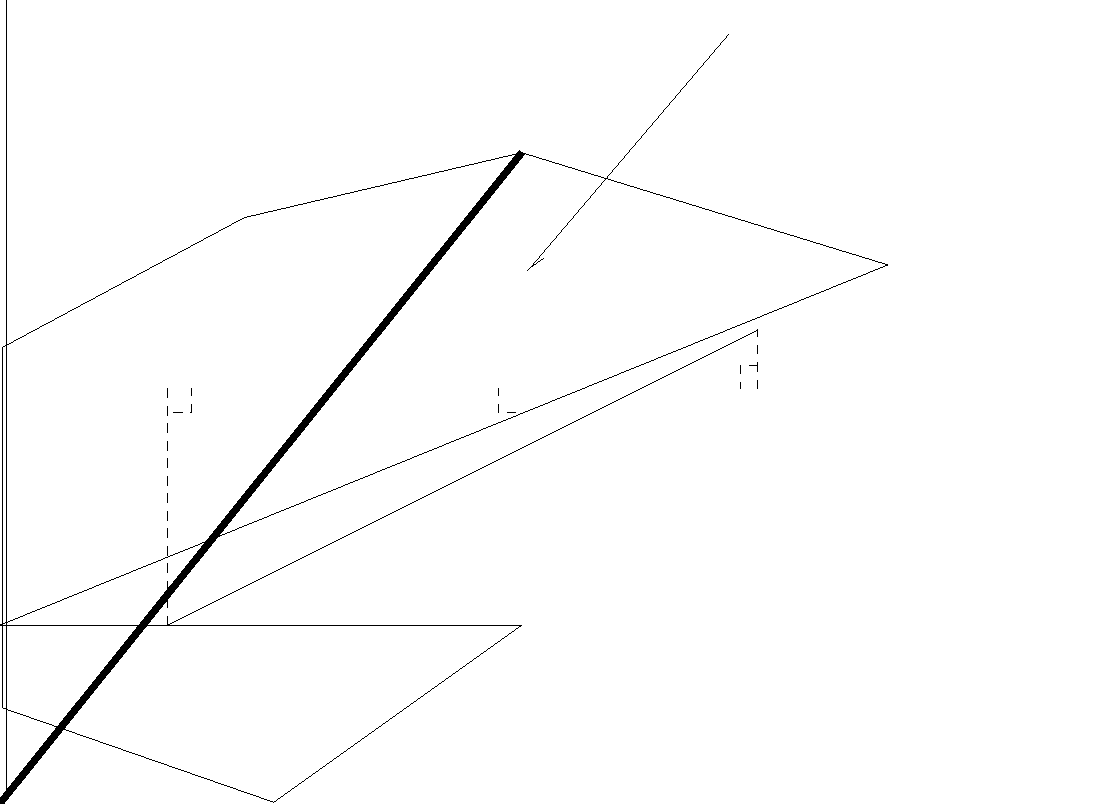
\includegraphics[height=4cm]{../Base/Bilsc2/Images/facette.pdf}}}
\parbox{8cm}{%
\centerline{
\includegraphics[height=4cm]{../Base/Bilsc2/Images/facebord.pdf}}}
\caption{\label{Base_Bilsc2_fig_geom}D\'efinition des diff\'erentes entit\'es
g\'eom\'etriques pour les faces internes (gauche) et de bord (droite).}
\end{figure}
\begin{equation}\notag
\displaystyle\alpha_{ij}=\frac{\overline{FJ'}}{\overline{I'J'}} \text{\ d\'efini aux faces internes uniquement et}
\end{equation}
\begin{equation}\notag
\vect{u}_{K'} = \vect{u}_{K}+(\ggrad{\vect{u}})_K\text{.}\, \vect{KK'}\, \text{\
\`a l'ordre 1 en espace, pour ${K = I \,\text{ou}\, J}$} 
\end{equation}\\ 
La valeur du flux convectif ${F_{\,ij}}$  d\'epend du type de sch\'ema num\'erique choisi. Il en existe trois dans ce sous-programme :


\renewcommand{\arraystretch}{2.}
\begin{tabular}{ll}
\multicolumn{2}{l}{$\bullet\ $un sch\'ema d\'ecentr\'e amont d'ordre 1 (upwind)~:}\\
&$F_{\,ij}((\rho \vect{u})^n,a)=
F^{\it{ amont}}_{\,ij}((\rho \vect{u})^n,a)$\\
o\`u :&
$a_{\,f,ij}= \left\lbrace\begin{array}{l}
a_I \text{ si }(\rho \vect{u})_{\,ij}^n\,.\,\vect{S}_{\,ij}\geqslant 0\\
a_J \text{ si }(\rho \vect{u})_{\,ij}^n\,.\,\vect{S}_{\,ij} < 0
\end{array}\right.$\\

\multicolumn{2}{l}{$\bullet\ $un sch\'ema centr\'e pur~:}\\
&$F_{\,ij}((\rho \vect{u})^n,a)=
F^{\text{\it{ centr\'e}}}_{\,ij}((\rho \vect{u})^n,a)$\\
avec :&$a_{\,f,ij}= \alpha_{ij} a_{I'}+(1-\alpha_{ij}) a_{J'}$\\
\multicolumn{2}{l}{$\bullet\ $un sch\'ema d\'ecentr\'e amont d'ordre 2, SOLU \footnotemark (Second Order Linear Upwind)~:}\\
&$F_{\,ij}((\rho \vect{u})^n,a)=
F^{\text{\it { SOLU}}}_{\,ij}((\rho \vect{u})^n,a)$ \\
avec :&
$a_{\,f,ij}=\left\lbrace\begin{array}{l}
a_I +\vect{IF}\,.\,(\grad a)_{\,I}
\text{\ \  si }(\rho \vect{u})_{\,ij}^n.\ \vect{S}_{\,ij}\geqslant 0\\
a_J + \vect{JF}\,.\,(\grad a)_{\,J}
\text{\ \  si }(\rho \vect{u})_{\,ij}^n.\ \vect{S}_{\,ij} < 0
\end{array}\right.$\\ 
\end{tabular}\\
\renewcommand{\arraystretch}{1.}
\footnotetext{Extrapolation de la valeur upwind au centre des faces.}

La valeur de $F_{\,b_{ik}}$ est calcul\'ee avec :
\begin{equation}\notag
{a_f}_{\,{b}_{ik}}=\left\lbrace\begin{array}{l}
a_I \text{ \ \ \ \ si }(\rho \vect{u})_{\,{b}_{ik}}^n
\text{.}\, \vect{S}_{\,{b}_{ik}}\geqslant 0\\
a_{\,{b}_{ik}}\text{ \ \ si } (\rho \vect{u})_{\,{b}_{ik}}^n
\text{.}\, \vect{S}_{\,{b}_{ik}} < 0
\end{array}\right.
\end{equation}
$a_{\,{b}_{ik}}$ est la valeur au bord donn\'ee directement par les
conditions aux limites.\\
 
\minititre{Remarque 1}
En sch\'ema centr\'e, on \'ecrit en r\'ealit\'e (\'egalit\'e
conservant l'ordre 1 en espace sur $a$) : 

\begin{equation}\notag
a_{\,f,ij} = \alpha_{ij} a_I +  (1-\alpha_{ij}) a_J  + \displaystyle
\frac{1}{2}\left[(\grad a)_I+(\grad a)_J\right] \text{.}\, \vect{OF}  
\end{equation}

On utilise le facteur $\displaystyle \frac{1}{2}$ pour des raisons purement de stabilit\'e num\'erique.\\\\
\minititre{Remarque 2}
Un test de pente qui peut introduire des non lin\'earit\'es dans l'op\'erateur
de convection permet de
basculer du sch\'ema centr\'e ou S.O.L.U. (d'ordre deux en maillage orthogonal)
vers le sch\'ema d\'ecentr\'e amont d'ordre un (sans blending). 
De plus, en mode standard, on utilise en tout point une valeur de 
$a_{\,f,ij}$ issue d'une moyenne barycentrique entre la valeur 
d\'ecentr\'ee amont et la valeur centr\'ee (blending), suivant le souhait de l'utilisateur (variable $\var{BLENCV}$ dans le sous-programme \fort{usini1}).


\subsection{\bf Partie diffusive}

De m\^eme, la partie diffusive peut s'\'ecrire (au signe pr\`es) :
\begin{equation}\notag
\int_{\Omega_i}{\dive(\,\beta\ \grad a)\  d\Omega} = 
\sum_{j\in Vois(i)}{D_{\,ij}(\,\beta, a)}
+\sum_{k\in {\gamma_b(i)}} {D_{\,{b}_{ik}}(\beta, a)}
\end{equation} 
avec~:
\begin{equation}
D_{\,ij}(\,\beta, a) = \beta_{\,ij}
\frac{a_{\,J'}- a_{\,I'}}{\overline{I'J'}} S_{\,ij} 
\end{equation}
et :
\begin{equation}
D_{\,b_{ik}}(\,\beta, a) = \beta_{\,b_{ik}}
\frac{a_{\,b_{ik}}-a_{\,I'}}{\overline{I'F}} S_{\,b_{ik}} 
\end{equation}
en conservant les notations pr\'ec\'edentes et avec $S_{\,ij}$ norme du vecteur
$\vect{S}_{\,ij}$, $S_{\,b_{ik}}$ norme du vecteur $\vect{S}_{\,b_{ik}}$,
${a_{\,{b}_{ik}}}$ valeur au bord donn\'ee directement par les conditions aux limites.\\
